
This section covers the description of the ``\Gls{NC} gamma'', or
single photon neutrino-production processes in more details. There is
no data that can constrain the cross section calculations that have
been made up to now, however some models are more theoretically
motivated than others. There are two main reasons why the \Gls{NCg}
interactions have an importance in the accelerator neutrino physics:
\begin{itemize}[noitemsep,topsep=0pt]
\item The background in the so-called \Gls{MiniBooNE} low-energy
  excess~\cite{MBexcess2009,AnuMiniBooNE2013}: This excess was
  discovered in the electron (anti-) neutrino samples of the
  \Gls{MiniBooNE} Cherenkov detector. \Gls{NCg} processes are one of
  the background for the electron (anti-) neutrino samples. The
  presence of these processes with cross section enhanced by a factor
  of 2.7 could explain this excess~\cite{MBexcess2009}.
\item The background for search for \Gls{CP} violation at \Gls{TK} or
  \Gls{NOvA}: Similarly to the \Gls{MiniBooNE} analyses, \Gls{NCg}
  events are one of the background for electron (anti-)
  neutrinos. From the last \Gls{TK} result~\cite{LastT2K}, it is clear
  that this background is already a problem.
\end{itemize}

The reason \Gls{NCg} events systematically are present in the electron
(anti-) neutrino samples was developed earlier, it is because the
photons and electrons produce the same signal in Cherenkov detectors
(see Section~\ref{subsubsec:ncgprocesses}).

Firstly, the models leading to these events are described, then the
generator implementation of the models are explained. Accurate
modeling of the \Gls{NCg} processes becomes increasingly important as
statistics in the electron sample increase and therefore the
statistical uncertainty on these becomes smaller. All the available
predictions (from generators and different theories) are summarised in
Figure~\ref{fig:integratedncg} for the integrated cross sections and
Figure~\ref{fig:diffncg} for simple one-dimensional differential cross
sections.

\begin{figure}[ht]
  \center
  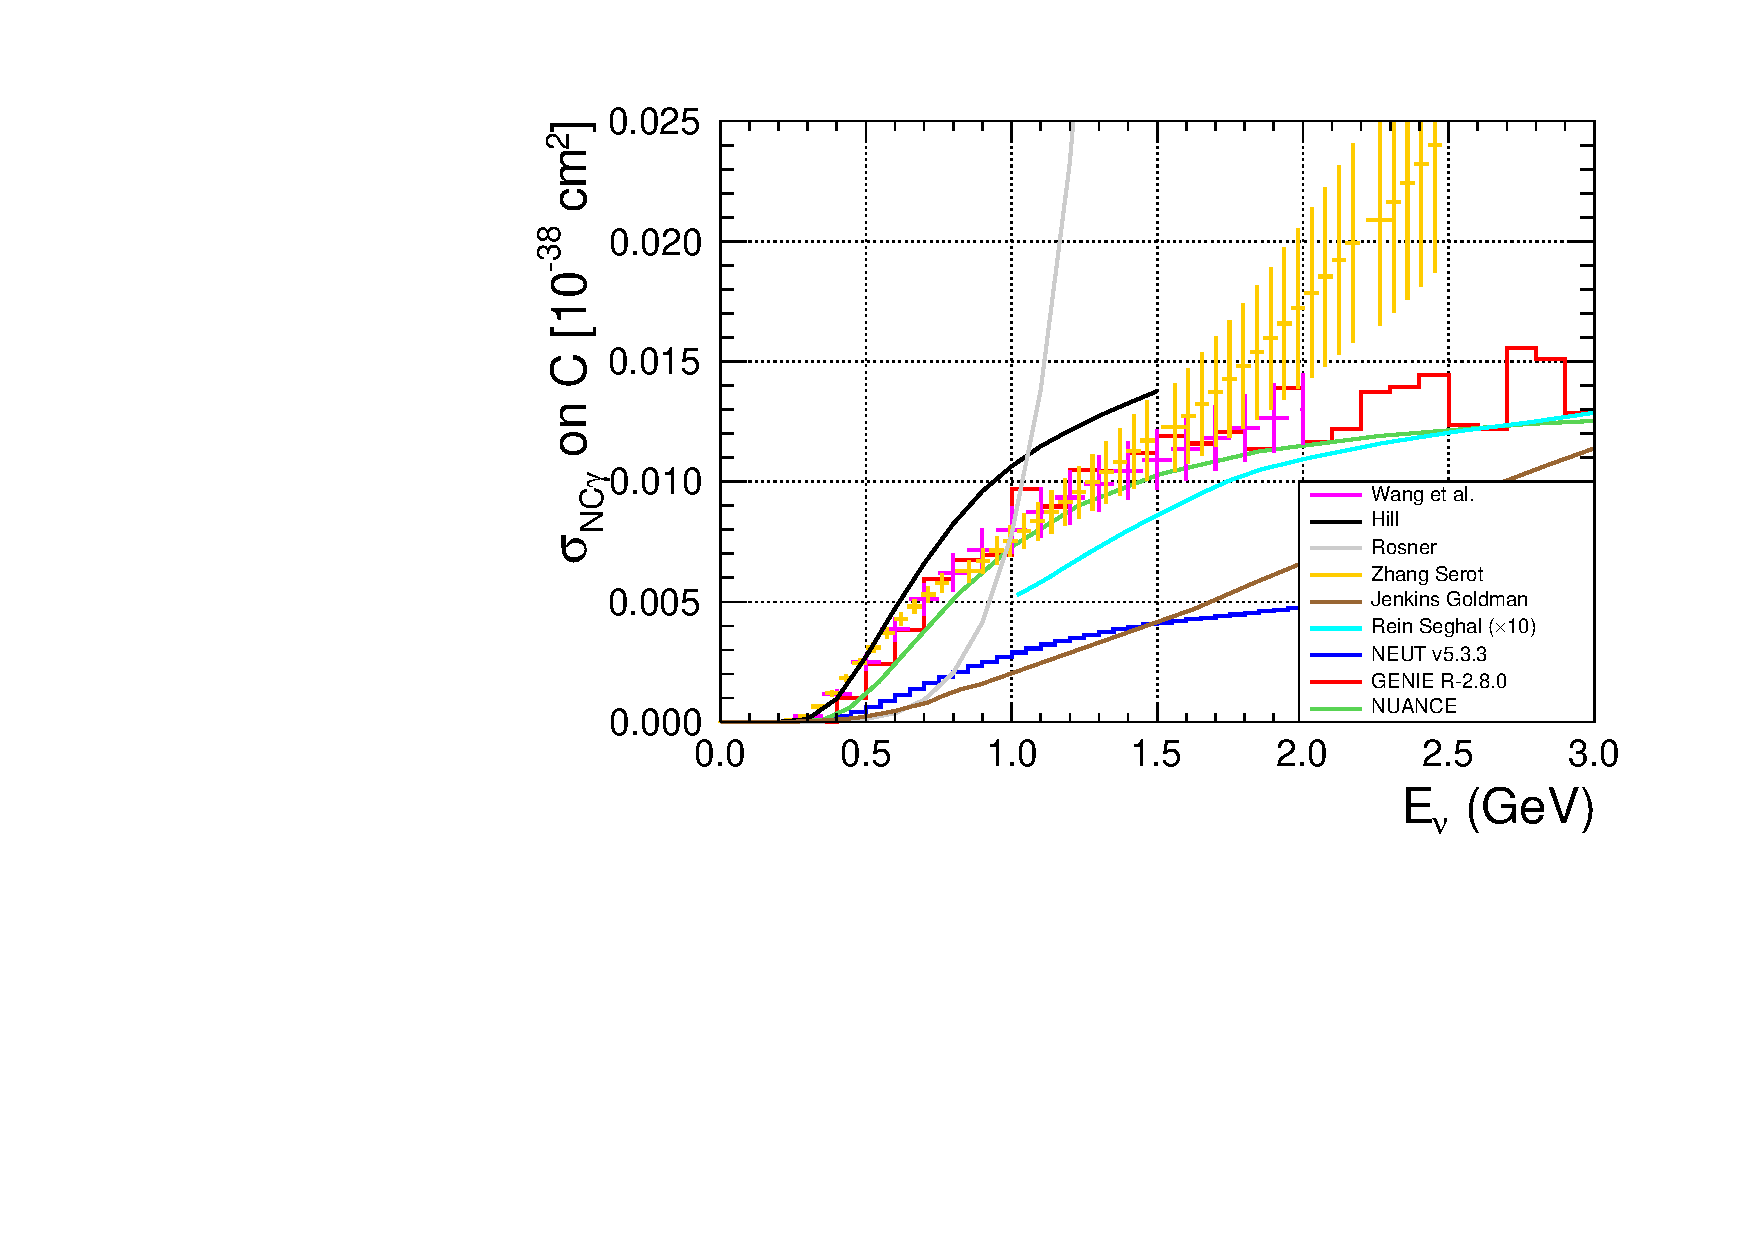
\includegraphics[width=0.68\textwidth]{images/Pheno/NCG_integrated.pdf}
  \caption[Integrated cross section for neutrino single photon
  production on carbon]{Integrated cross section for neutrino single
    photon production on carbon, based on the theoretical work from:
    Wang~et~al.~\cite{Alvarez2014}, Hill~\cite{Hills2007},
    Rosner~\cite{Rosner2015}, Zhang~et~al.~\cite{Serot2012}, Jenkins
    Goldman~\cite{Jenkins}, Rein Seghal~\cite{ReinCohGamma}. The
    following are neutrino interaction generators:
    \Gls{NEUT}~\cite{NEUT}, \Gls{GENIE}~\cite{GENIE1,GENIE2} and
    \Gls{NUANCE}~\cite{nuance}. Figure based on~\cite{Garvey:2014exa}
    (Figure~43).}
  \label{fig:integratedncg}
\end{figure}

\begin{figure}[ht]
  \center
  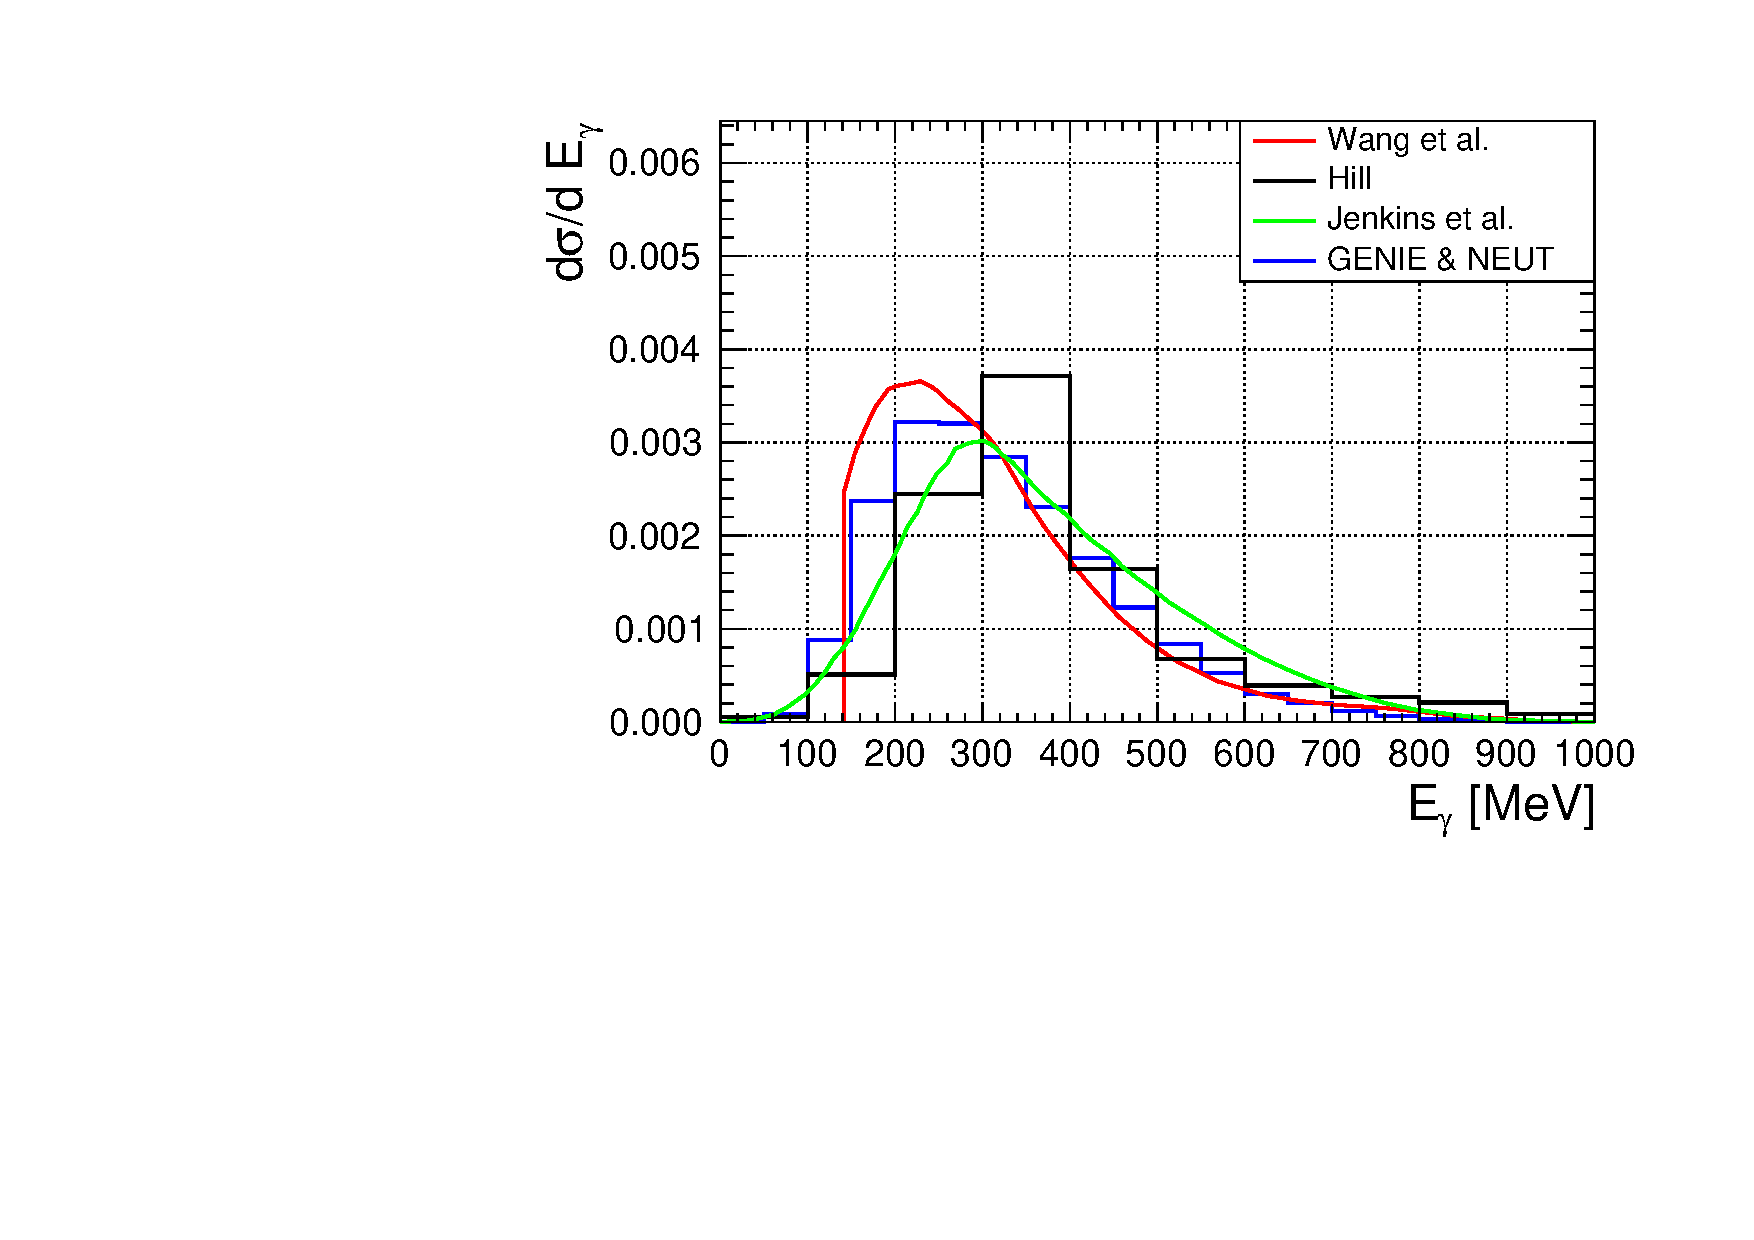
\includegraphics[width=0.7\textwidth]{images/Pheno/NCG_Diff_ene.pdf}
  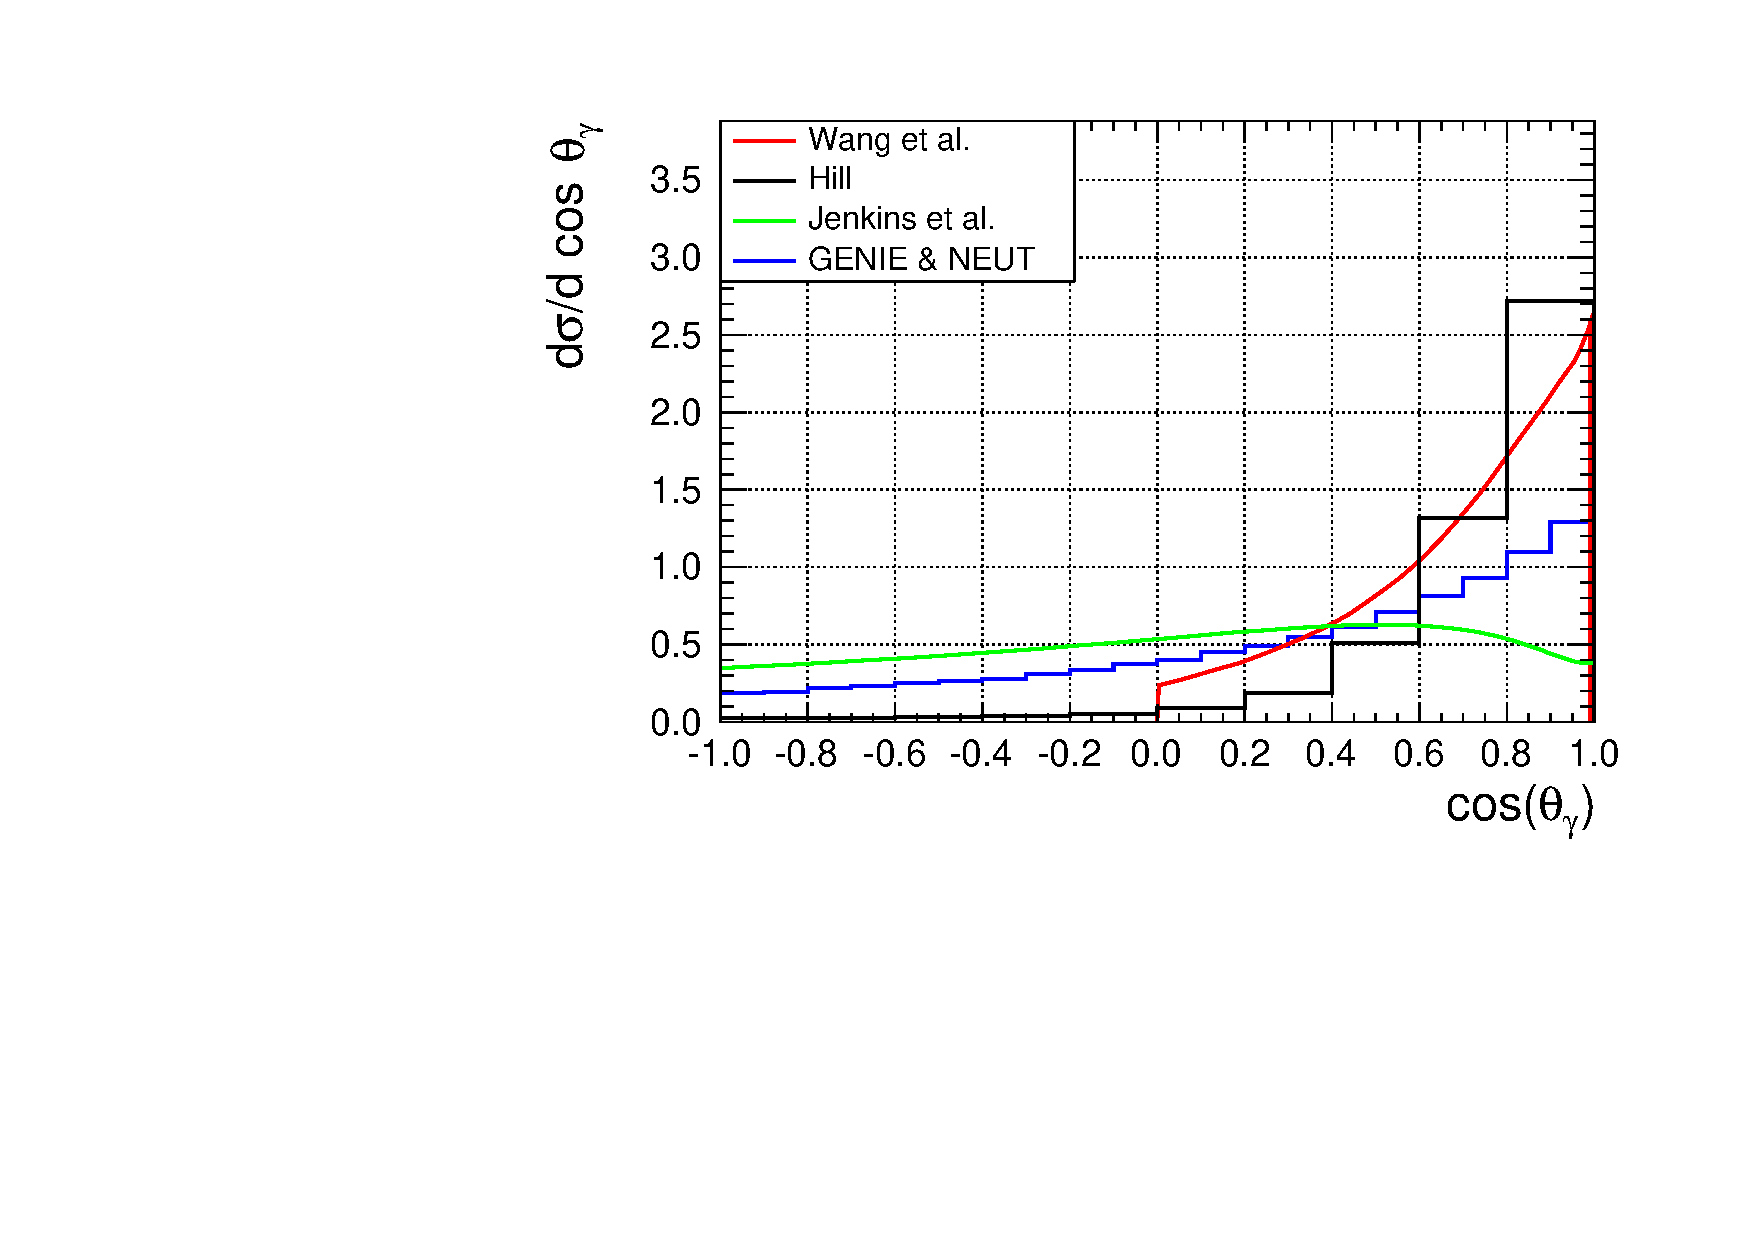
\includegraphics[width=0.7\textwidth]{images/Pheno/NCG_Diff_cos.pdf}
  \caption[Differential cross sections for a 1~GeV neutrino single
  photon production on carbon]{Differential cross sections for a
    $1$~GeV neutrino single photon production on
    carbon. \textbf{\textit{Top:}} Differential cross section in
    photon energy. \textbf{\textit{Bottom:}} Differential cross
    section in photon angle (right), based on the theoretical work
    from: Wang~et~al.~\cite{Alvarez2014}, Hill~\cite{Hills2007},
    Jenkins Goldman~\cite{Jenkins}, \Gls{NEUT}~\cite{NEUT}. The
    following are neutrino interaction generators:
    \Gls{GENIE}~\cite{GENIE1,GENIE2}. All the distributions have been
    normalised to unit area. The \Gls{NEUT} and \Gls{GENIE}
    distributions are almost identical, so only the \Gls{NEUT}
    distribution was kept for clarity.}
  \label{fig:diffncg}
\end{figure}
\clearpage

\section{Models}
\label{sec:models}

Figure~\ref{fig:FeynmanDiagramNCG} shows the Feynman diagrams that are
used in recent
calculations~\cite{Alvarez2014,Hills2007,Rosner2015,Serot2012,Jenkins,ReinCohGamma}. All
the models use a resonant production model based on the chiral
description of the nucleus, except the Rein and Sehgal model which
only has the coherent contribution. Note that this is a different
model to the one that is implemented in the generators.

The model in~\cite{Alvarez2014} carefully estimates the
background~/~$\Delta$~/~higher resonances interferences by adding
coherently all the amplitudes of the Feynman diagrams in
Figure~\ref{fig:FeynmanDiagramNCG} (contribution 1 to 6). The model in
\cite{Hills2007} takes into account a the $\Delta$ contribution (1 in
the figure), and an additional anomalous countribution (9 in the
figure) All the known effects due to the nuclear medium are also taken
into account.  Figure~\ref{fig:diffncg} shows the differential one
dimensional cross section available for the \Gls{NCg}.

\begin{figure}[ht]
  \center
  \textbf{\textit{1)}}\hspace{1cm}\begin{fmffile}{feynmandiag/directdelta}
    \begin{fmfgraph*}(27,27)
      \fmfstraight
      \fmftop{i2,o3}
      \fmfleft{i1,b2,b3,i2}
      \fmfright{o1,o2,o3}
      \fmfbottom{i1,o1}
      \fmf{fermion,tension=1.5}{i2,v1}
      \fmflabel{$\nu$}{i2}
      \fmf{fermion}{v1,o3}
      \fmflabel{$\nu$}{o3}
      \fmf{fermion,tension=1.7}{i1,v2}
      \fmflabel{$n/p$}{i1}
      % \fmfstraight
      \fmf{dbl_plain_arrow,label=$\Delta$,tension=2}{v2,v3}
      \fmf{photon,label=$Z^0$}{v1,v2}
      \fmf{photon,tension=1.5}{v3,o2}
      \fmflabel{$\gamma$}{o2}
      \fmf{fermion}{v3,o1}
      \fmflabel{$n/p$}{o1}
    \end{fmfgraph*}
  \end{fmffile} 
  \hspace{2cm}
  \textbf{\textit{2)}}\hspace{1cm}\begin{fmffile}{feynmandiag/indirectdelta}
    \begin{fmfgraph*}(27,27)
      \fmfstraight
      \fmftop{i2,o4}
      \fmfleft{i1,b2,b3,i2}
      \fmfright{o1,o2,o3,o4}
      \fmfbottom{i1,o1}
      \fmf{fermion,tension=2}{i2,v1}
      \fmflabel{$\nu$}{i2}
      \fmf{fermion}{v1,o4}
      \fmflabel{$\nu$}{o4}
      \fmf{fermion,tension=3}{i1,v2}
      \fmflabel{$n/p$}{i1}
      % \fmfstraight
      \fmf{dbl_plain_arrow,label=$\Delta$}{v2,v3}
      \fmf{photon}{v1,v3}
      % \fmflabel{$Z^0$}{v1}
      \fmf{photon,tension=1.4}{v2,o3}
      \fmflabel{$\gamma$}{o3}
      \fmf{fermion,tension=3}{v3,o1}
      \fmflabel{$n/p$}{o1}
      \fmffreeze
      \fmf{phantom,label.dist=0,label=$Z^0$}{v1,o3}
    \end{fmfgraph*}
  \end{fmffile}

  \vspace{1cm}
  \textbf{\textit{3)}}\hspace{1cm}\begin{fmffile}{feynmandiag/directother}
    \begin{fmfgraph*}(27,27)
      \fmfstraight
      \fmftop{i2,o3}
      \fmfleft{i1,b2,b3,i2}
      \fmfright{o1,o2,o3}
      \fmfbottom{i1,o1}
      \fmf{fermion,tension=1.5}{i2,v1}
      \fmflabel{$\nu$}{i2}
      \fmf{fermion}{v1,o3}
      \fmflabel{$\nu$}{o3}
      \fmf{fermion,tension=1.7}{i1,v2}
      \fmflabel{$n/p$}{i1}
      % \fmfstraight
      \fmf{dbl_plain_arrow,label=$N^*$,tension=2}{v2,v3}
      \fmf{photon,label=$Z^0$}{v1,v2}
      \fmf{photon,tension=1.5}{v3,o2}
      \fmflabel{$\gamma$}{o2}
      \fmf{fermion}{v3,o1}
      \fmflabel{$n/p$}{o1}
    \end{fmfgraph*}
  \end{fmffile}
  \hspace{2cm} 
  \textbf{\textit{4)}}\hspace{1cm}\begin{fmffile}{feynmandiag/indirectother}
    \begin{fmfgraph*}(27,27)
      \fmfstraight
      \fmftop{i2,o4}
      \fmfleft{i1,b2,b3,i2}
      \fmfright{o1,o2,o3,o4}
      \fmfbottom{i1,o1}
      \fmf{fermion,tension=2}{i2,v1}
      \fmflabel{$\nu$}{i2}
      \fmf{fermion}{v1,o4}
      \fmflabel{$\nu$}{o4}
      \fmf{fermion,tension=3}{i1,v2}
      \fmflabel{$n/p$}{i1}
      % \fmfstraight
      \fmf{dbl_plain_arrow,label=$N^*$}{v2,v3}
      \fmf{photon}{v1,v3}
      % \fmflabel{$Z^0$}{v1}
      \fmf{photon,tension=1.4}{v2,o3}
      \fmflabel{$\gamma$}{o3}
      \fmf{fermion,tension=3}{v3,o1}
      \fmflabel{$n/p$}{o1}
      \fmffreeze
      \fmf{phantom,label.dist=0,label=$Z^0$}{v1,o3}
    \end{fmfgraph*}
  \end{fmffile}

  \vspace{1cm}
  \textbf{\textit{5)}}\hspace{1cm}\begin{fmffile}{feynmandiag/directnucleon}
    \begin{fmfgraph*}(27,27)
      \fmfstraight
      \fmftop{i2,o3}
      \fmfleft{i1,b2,b3,i2}
      \fmfright{o1,o2,o3}
      \fmfbottom{i1,o1}
      \fmf{fermion,tension=1.5}{i2,v1}
      \fmflabel{$\nu$}{i2}
      \fmf{fermion}{v1,o3}
      \fmflabel{$\nu$}{o3}
      \fmf{fermion,tension=1.7}{i1,v2}
      \fmflabel{$n/p$}{i1}
      % \fmfstraight
      \fmf{fermion,label=$n/p$,tension=2}{v2,v3}
      \fmf{photon,label=$Z^0$}{v1,v2}
      \fmf{photon,tension=1.5}{v3,o2}
      \fmflabel{$\gamma$}{o2}
      \fmf{fermion}{v3,o1}
      \fmflabel{$n/p$}{o1}
    \end{fmfgraph*}
  \end{fmffile}
  \hspace{2cm} 
  \textbf{\textit{6)}}\hspace{1cm}\begin{fmffile}{feynmandiag/indirectnucleon}
    \begin{fmfgraph*}(27,27)
      \fmfstraight
      \fmftop{i2,o4}
      \fmfleft{i1,b2,b3,i2}
      \fmfright{o1,o2,o3,o4}
      \fmfbottom{i1,o1}
      \fmf{fermion,tension=2}{i2,v1}
      \fmflabel{$\nu$}{i2}
      \fmf{fermion}{v1,o4}
      \fmflabel{$\nu$}{o4}
      \fmf{fermion,tension=3}{i1,v2}
      \fmflabel{$n/p$}{i1}
      % \fmfstraight
      \fmf{fermion,label=$n/p$}{v2,v3}
      \fmf{photon}{v1,v3}
      % \fmflabel{$Z^0$}{v1}
      \fmf{photon,tension=1.4}{v2,o3}
      \fmflabel{$\gamma$}{o3}
      \fmf{fermion,tension=3}{v3,o1}
      \fmflabel{$n/p$}{o1}
      \fmffreeze
      \fmf{phantom,label.dist=0,label=$Z^0$}{v1,o3}
    \end{fmfgraph*}
  \end{fmffile}

  \vspace{1cm}
  \textbf{\textit{7)}}\hspace{1cm}\begin{fmffile}{feynmandiag/pionex}
    \begin{fmfgraph*}(27,27)
      \fmfstraight
      \fmftop{i2,o4}
      \fmfleft{i1,b2,b3,i2}
      \fmfright{o1,o2,o3}
      \fmfbottom{i1,o1}
      \fmf{fermion}{i2,v1}
      \fmflabel{$\nu$}{i2}
      \fmf{fermion}{v1,o4}
      \fmflabel{$\nu$}{o3}
      \fmf{fermion}{i1,v3}
      \fmflabel{$n/p$}{i1}
      % \fmfstraight
      \fmf{photon,label=$Z^0$}{v1,v2}
      \fmf{dashes,label=$\pi^0/\omega^0/\rho^0$}{v2,v3}
      % \fmflabel{$Z^0$}{v1}
      \fmf{photon}{v2,o2}
      \fmflabel{$\gamma$}{o2}
      \fmf{fermion}{v3,o1}
      \fmflabel{$n/p$}{o1}
    \end{fmfgraph*}
  \end{fmffile}
  \hspace{2cm} 
  \textbf{\textit{8)}}\hspace{1cm}\begin{fmffile}{feynmandiag/contact}
    \begin{fmfgraph*}(27,27)
      \fmfstraight
      \fmftop{i2,o4}
      \fmfleft{i1,b2,b3,i2}
      \fmfright{o1,o2,o3}
      \fmfbottom{i1,o1}
      \fmf{fermion}{i2,v1}
      \fmflabel{$\nu$}{i2}
      \fmf{fermion}{v1,o4}
      \fmflabel{$\nu$}{o3}
      \fmf{fermion,tension=1.5}{i1,v2}
      \fmflabel{$n/p$}{i1}
      % \fmfstraight
      \fmf{photon,label=$Z^0$}{v1,v2}
      % \fmflabel{$Z^0$}{v1}
      \fmf{photon}{v2,o2}
      \fmflabel{$\gamma$}{o2}
      \fmf{fermion}{v2,o1}
      \fmflabel{$n/p$}{o1}
    \end{fmfgraph*}
  \end{fmffile}

  \vspace{1cm}
  \textbf{\textit{9)}}\hspace{1cm}\begin{fmffile}{feynmandiag/anomaly}
    \begin{fmfgraph*}(27,27)
      \fmfstraight
      \fmftop{i2,o4}
      \fmfleft{i1,b2,b3,i2}
      \fmfright{o1,o2,o3}
      \fmfbottom{i1,o1}
      \fmf{fermion}{i2,v1}
      \fmflabel{$\nu$}{i2}
      \fmf{fermion}{v1,o4}
      \fmflabel{$\nu$}{o3}
      \fmf{fermion}{i1,v3}
      \fmflabel{$n/p$}{i1}
      % \fmfstraight
      \fmf{photon,label=$Z^0$}{v1,v4}
      \fmf{dashes,label=$\omega^0$}{v5,v3}
      % \fmflabel{$Z^0$}{v1}
      \fmf{photon}{v6,o2}
      \fmf{fermion,tension=0.5}{v4,v5,v6,v4}
      \fmflabel{$\gamma$}{o2}
      \fmf{fermion}{v3,o1}
      \fmflabel{$n/p$}{o1}
    \end{fmfgraph*}
  \end{fmffile}
  
  \caption[Feynman diagrams contributing to the neutrino production of
    a single photon]{Feynman diagrams contributing to the neutrino production of
    a single photon:
    \textbf{\textit{1)}} Direct $\Delta$ excitation.
    \textbf{\textit{2)}} Crossed $\Delta$ excitation.
    \textbf{\textit{3)}} Direct heavy resonance excitation.
    \textbf{\textit{4)}} Crossed heavy resonant excitation.
    \textbf{\textit{5)}} Direct nucleon excitation (or
    ``background'').
    \textbf{\textit{6)}} Crossed nucleon excitation.
    \textbf{\textit{7)}} Meson exchange.
    \textbf{\textit{8)}} Contact.
    \textbf{\textit{9)}} Anomaly mediated.}
  \label{fig:FeynmanDiagramNCG}
\end{figure} 

\clearpage

\section{Generators}
\label{sec:generator}
The two main generators (\Gls{NEUT}~\cite{NEUT} and
\Gls{GENIE}~\cite{GENIE1,GENIE2}) used for accelerator and atmospheric
neutrino experiments use a similar way to treat the \Gls{NCg}
processes. They rely on the ``standard'' Rein and Seghal resonance
production from neutrino interaction~\cite{Rein1}. As was the case in
the \Gls{RES} section~(\ref{subsec:res}), the cross sections are
computed via a differential $\frac{d^2\sigma}{dQ^2dW_{inv}}$
calculation. Note that these are free nucleon calculations. The only
nuclear effects taken into account are the Fermi momentum of the
struck nucleon and the Pauli blocking, and the final state effects for
the outgoing nucleons. The photon does not undergo final state
interactions, unlike a typical pion production. One of the main
differences between \Gls{NEUT} and \Gls{GENIE} is the fact that the
\Gls{NEUT} adds all the resonance contributions at the amplitude
level, thus considering all the interferences between
them. \Gls{GENIE} adds all the contributions incoherently.

The main problem with \Gls{GENIE} and \Gls{NEUT}'s approach is that
the invariant mass has no effect on the decays branching ratios of the
resonance. This is quite counter-intuitive since there is, a priori,
no restriction on the lower limit for the invariant mass, which could
be smaller than the mass of a pion and a nucleon, and would therefore
lead to an enhancement of the ``NC gamma'' cross section in this
region of phase space. This problem was overcome in
\Gls{NUANCE}~\cite{nuance}, the generator used for the \Gls{MiniBooNE}
experiment, where the branching ratio was manually changed for small
$W$.

The other main problem is the absence of coherent effects in the
generators, which is a contribution of around $10~\%$ to the total
cross section that has been neglected.

Finally, it was noted that a bug was present in \Gls{NEUT}: the
branching ratios were wrong and producing 1/2 of the expected cross
section~\cite{Kendall2015}. This is visible in
Figure~\ref{fig:integratedncg}. Note that this bug marginally impacts
the differential cross section and therefore has a no effect on the
result discussed in this thesis. This is because \Gls{NEUT} is only
used to calculate the efficiency of the \Gls{NCg} events as will be
discussed in a subsequent chapter.



\section{Summary}
\label{sec:phenosummary}
In this chapter, the predictions of the models leading to the
neutrino-production of single photons are shown and explained. The
conclusion is that the cross section for such events is much smaller
than the cross section of dominant processes in \Gls{TK}
(\Gls{CCQE}). The \Gls{NCg} cross section is roughly three orders of
magnitude smaller than the one of \Gls{CCQE} at 1~GeV.

The absence of any measurement for \Gls{NCg} processes leads to high
uncertainties in the theoretical predictions and it is impossible to
conclude which model is more suitable.














